%
% chap001.tex
%

%======================================================
\chapter{Primzahlen}
%======================================================

%======================================================
\section{Primzahlbegriff und geschichtliche Aspekte}
%======================================================
\begin{definition}[Primzahl]
``Eine Primzahl ist eine natürliche Zahl $p > 1$, die nur 
die trivialen Teiler besitzt, d.h. deren einzige Teiler
1 und sie selbst sind'' (\cite{schichlsteinbauer}, S.23).
\end{definition}
\vspace{-.5cm}

\begin{minipage}{0.65\linewidth}
Die Primzahlen sind nicht vor einer kurzen Zeit erfunden
worden. Schon vor mehrere hunderte von Jahren hatten sich
die Mathematiker mit den Primzahlen beschäftigt.
Hinsichtlich der Mathematiker, die als erste die Primzahlen
untersuchten, sind die Mathematiker der pythagoräischen
Schule (ab 500 bis 300 v. Chr.). Sie fokussierten sich auf
die perfekten und befreundeten Zahlen und infolgedessen
untersucheten sie die Primzahlen, aber auch die
zusammengesetzten Zahlen. Es wurden viele relevante
Entdeckungen von ihnen gemacht, jedoch konnten sie ihre
Theorien nicht beweisen.
\end{minipage}
\hfil
\begin{minipage}[r]{0.3\linewidth}
  % insert this 2 lines before \includegraphics to avoid the warning "the option `hypcap=true' will be ignored for this particular \caption on input line.
  % This warning occurs, because a conflict at paramter "hypcap=true" when load both packages "hyperref" and "caption".
  %\captionsetup[figure]{labelformat=empty}% turn off figure prefix "Figure:" or "Abbildung"
  \captionsetup{type=figure,font=small,skip=6pt,format=plain}% {format=hand}
  \capstart
  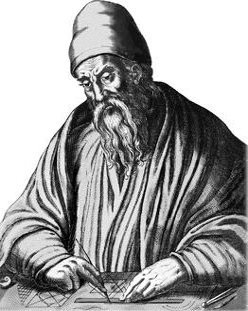
\includegraphics[width=1.0\linewidth]{./images/euklid.jpg}
  \captionof{figure}[Bild von Euklid. (Kurz-Info: Euklid und die Elemente,
2021)]{Bild von Euklid}
  \label{fig:portrait_euklid}
\end{minipage}
\vspace{.3cm}

``Um 300 v. Chr. veröffentlichte Euklid die Bücher der
”Elemente“, die viele wichtige Erkenntnisse der Primzahlforschung
mit korrekt geführten Beweisen beinhalteten''
(vgl. \cite{sasgabor}, S.4).
Einer der wichtigen Beweise sind die unendlich vielen Primzahlen.

\begin{theorem}[Satz von Euklid]
Es gibt unendlich viele Primzahlen.
\end{theorem}
\vspace{-.7cm}

\begin{proof}
Angenommen gäbe es nur endlich viele Primzahlen.
So bezeichnet man sie mit $p_1 ,...,p_n$ und $n$
ist die endliche Anzahl von Primzahlen.
Also bildet man die Zahl $m = p_1 p_2 \dots p_n + 1$.
``Weiters verwenden wir die Tatsache, dass jede 
natürliche Zahl größer $1$ in Primfaktoren zerlegt, 
d.h. als Produkt von Primzahlen geschrieben werden kann''.
Jede solche Zahl ist durch mindestens eine Primzahl teilbar.
Hinsichtlich dieser Tatsache muss es eine Primzahl geben, 
die $m$ teilt. ``Dies ist jedoch nicht möglich, da $m$
durch keine der Primzahlen $p_i$ $(1 \leq i \leq n)$ teilbar
ist. (Es bleibt ja immer ein Rest von 1)''. Die logische
Schlusskette endet in einem Widerspruch
(vgl. \cite{schichlsteinbauer}, S.25).
\end{proof}

\newpage


\textbf{CHINESISCHE VERMUTUNG}

Ungefähr um die Lebzeit von Konfuzius ist eine Vermutung
aufgestellt worden, die besagt, dass eine Zahl $n$ dann
und nur dann eine Primzahl ist, falls diese $2^{n} - 2$
teilt. Diese Vermutung stellte sich aber falsch heraus,
denn $2^{341} - 2$ ist durch $341$ teilbar und $341$ ist
eine zusammengesetzte Zahl. Häufig gab es Bezweiflungen,
ob die Chinesen diese Vermutung tatsächlich aufgestellt
hätten und man dachte auch, dass sie das Konzept der
Primzahlen nie verfasst haben.

Diese Vermutung wird als Chinesische Hypothese bezeichnet
(vgl. \cite{sasgabor}, S.4ff). 
\vspace*{.4cm}

\textbf{SIEB DES ERATOSTHENES}

Um 200 v. Chr. erfand Eratosthenes einen Algorithmus zur
Anfertigung einer Tabelle mit allen Primzahlen bis zu
einer bestimmten Zahl. Seine Methode wurde nach ihm
benannt und sie heißt heute ''Sieb des Eratosthenes``
(vgl. \cite{sasgabor}, S.5).
\vspace*{.4cm}

\underline{Kurze Erklärung zur Funktionsweise des Algorithmus}

Zu Beginn wird eine Liste bestehend aus natürlichen Zahlen
erstellt. Die Liste beginnt mit $2$ und endet bei einer
gewünschten Zahl $n$. Es wird die erste Zahl (die $2$)
durch das Umkreisen markiert und alle Vielfachen von $2$
werden durchgestrichen. Danach wird die nächste nicht
durchgestrichene Zahl, also die $3$ markiert und ebenfalls
die Vielfachen von $3$ durchgestrichen. Diese Methode wird
solange fortgesetzt, bis tatsächlich nur noch Zahlen in der
Liste überbleiben, die markiert sind bzw. die keine Teiler
(abgesehen von $1$ und sich selbst) aufweisen. Diese Zahlen
sind die Primzahlen. Alle durchgestrichenen Zahlen sind die
Vielfachen von den markierten Zahlen und diese sind teilbar
(vgl. \cite{sasgabor}, S.5).

\begin{figure}[H]
  \centering
  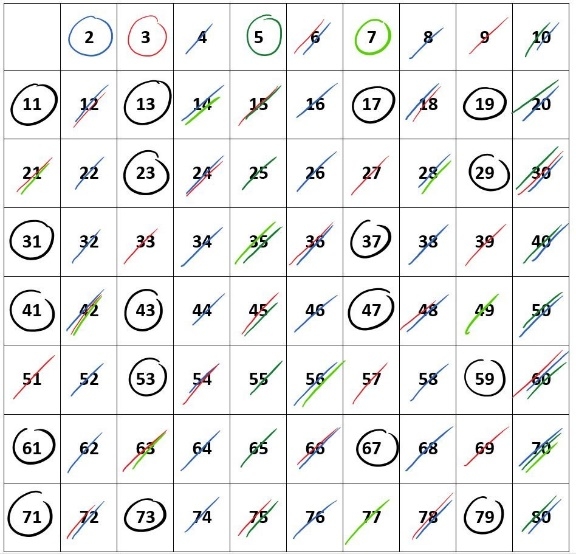
\includegraphics[width=.5\linewidth]{./images/sieb.jpg}
  \caption[Das Sieb des Eratosthenes. Abgerufen am 2021 von Serlo, die freie Lernplattform:
https://de.serlo.org/mathe/96712/das-sieb-des-eratosthenes]{Sieb des Eratosthenes}
  \label{fig:sieb_eratosthenes}
\end{figure}
\vspace{.2cm}

Diese Technik ist bis zu einer bestimmten Zahl zwar gut
gedacht, jedoch ist sie als Primzahltest nicht geeignet.
''Um die Primalität einer Zahl $n$ mit dem Sieb von
Eratosthenes festzustellen, muß die Primalität aller
Zahlen kleiner als $n$ festgestellt werden``
(siehe \cite{sasgabor}, S.5).
\vspace*{.4cm}

\textbf{MERSENNEZAHLEN UND DER KLEINE FERMATSCHE SATZ}

Lange Zeit nach Eratosthenes wurde keine mathematische
Forschung betrieben. Man begann sich mit der Mathematik
und somit auch mit den Primzahlen wieder währende der 
Renaissance zu beschäftigen. ''Dabei mussten viele
Erkenntnisse aus der Zeit der Griechen erst wieder neu
entdeckt werden``. Bezüglich der ersten Erforschungen
der Neuzeit wurden die Zahlen der Form $2^{n}-1$
untersucht und diese Zahlen werden Mersennezahlen genannt.
Die abgekürzte Form ist $M_n$. ''Es ist leicht zu zeigen,
daß $n$ prim sein muß, damit $M_n$ prim sein kann, daß
nicht alle Zahlen dieser Form mit einer Primzahl $n$
wieder eine Primzahl ist, wurde 1536 entdeckt 
($211 - 1 = 2047 = 23 \cdot 89$)``. Im Jahr 1588 wurde von
Cataldi bewiesen, dass $2^{19} - 1$ eine Primzahl ist
und sie blieb ungefähr 200 Jahre lang die größte Primzahl
(vgl. \cite{sasgabor}, S.6f).

Zu Beginn des 17. Jahrhundert hat Fermat die erste
wirklich andeutende Entdeckung seit Eratosthenes gemacht
und eine neue Technik zur Zerlegung von größeren Zahlen
gefunden. Hinsichtlich der Primzahlen gibt es den bekannten
und nach ihm benannten Kleinen Fermatschen Satz, der besagt,
dass falls $p$ eine Primzahl ist, gilt für jede ganze Zahl
$a$, daß $a^p \equiv a \mskip-5mu\mod p$. Dieser Satz unterstütz als
Grundidee viele weitere Erkenntnisse in der Zahlentheorie
und zahlreiche von Computern verwendete Verfahren zum
Überprüfen von Primzahlen beziehen sich auf diesen Satz
(vgl. \cite{sasgabor}, S.6f).
\vspace*{.4cm}

\textbf{DIE ZEIT AB DEM 20. JAHRHUNDERT}

Ab Mitte des 20. Jahrhunderts haben die Computer in der
Wissenschaft und auch in der Mathematik eine wichtige
Rolle gespielt. Zwar hat diese neue Technik kaum neue
Erkenntnisse hinsichtlich des Gebietes der Zahlentheorie
gebracht, aber einen Primzahlrekord nach dem anderen.
Der Amerikaner Robinson war der erste, den Computer zum
Finden von Primzahlen verwendete und $M_{2281}$ war die
größte Primzahl, die er fand. Diese Entdeckung passierte
im Jahr 1952. In den weiteren Jahren bzw. in der Folgezeit
sind alle paar Jahre ein neuer Rekord gefunden worden
(vgl. \cite{sasgabor}, S.7f).

Im Rahmen des Projekts Great Internet Mersenne Prime Search
(GIMPS) ist im Jahr 2018 die aktuell größte Primzahl
$M_{82589933}$ entdeckt worden. Der US-amerikanische
IT-Fachmann Patrick Laroche identifizierte die neue größte
Primzahl mit ungefähr 25 Millionen Stellen und diese Zahl
ist um mehr als 1,5 Millionen Ziffern länger als der
bisherige Rekordhalter
(vgl. \cite{derstandard}, 2018)
\newpage


%======================================================
\section{Primzahltests}
%======================================================

Wie im ersten Unterkapitel beschrieben, sind die Primzahlen
unendlich. Das heißt, dass es auch große Primzahlen
existieren, die für viele Verschlüsselungsverfahren immens
bedeutend sind.

Jedoch gibt es keine Konstruktionsmethode hinsichtlich der
Primzahlen, etwa wie eine effizient berechenbare Funktion
$f : \mathbb{N} \to \mathbb{P}$ mit unendlicher Bildmenge
(vgl. \cite{karpfingerkiechle}, S.141).
In diesem Abschnitt ist $\mathbb{P}$ die Menge aller
Primzahlen.

In der Praxis wird eine ungerade natürliche Zahl $n$
ausgesucht und auf Primalität geprüft. Es wird also geprüft,
ob die Zahl $n$ eine Primzahl ist und dazu werden die
Primzahltests benutzt. Wird anhand eines solchen Tests
festgestellt, dass die Zahl $n$ keine Primzahl ist, so
wird eine zu $n$ nächstgelegene ungerade natürliche Zahl
überprüft. Der Primzahlsatz garantiert dabei, dass mit
hoher Wahrscheinlichkeit in der Nähe von $n$ eine Primzahl
liegt (vgl. \cite{karpfingerkiechle}, S.141).
Des Weiteren definiert der Primzahlsatz eine asymptotische
Aussage über die Anzahl der Primzahlen (vgl. \cite{schuerz}, S.3).

\begin{theorem}[Primzahlsatz]
Es gilt \( \pi (x) \sim \frac{x}{\log(x)}\), d.h.
\( \lim\limits_{x\to\infty} \pi(x)\cdot \frac{\log(x)}{x} = 1 \)
(vgl. \cite{karpfingerkiechle}, S.142).
\end{theorem}

\textbf{ARTEN VON PRIMZAHLTESTS}
\begin{itemize}
 \item \textbf{Echte Primzahltests}\\
    Die echten Primzahltests definieren bzw. erkennen immer,
    ob eine Zahl zusammengesetzt oder prim ist. Des Weiteren
    beziehen sich diese Tests auf Aussagen der Art ''$n$ ist
    genau dann eine Primzahl, falls folgende Bedingungen
    gelten`` (vgl. \cite{sasgabor}, S.10). Anhand der echten
    Primzahltests wie beispielsweise die Probedivision,
    Sieb des Eratosthenes und Sieb von Atkin können mögliche
    Teiler einfach gefunden werden (vgl. \cite{primzahltest}, 2021).
    
 \item \textbf{Tests auf Zusammengesetztheit}\\
    Bestätigt ein Test dieser Form das Ergebnis
    ''zusammengesetzt``, so ist die zu prüfende Zahl mit
    Sicherheit zusammengesetzt. Es kann aber nicht davon
    ausgegangen werden, dass falls man nicht zusammengesetzt
    bekommt, dass die Zahl auch tatsächlich eine Primzahl ist.
    Die Tests auf Zusammengesetztheit beziehen sich auf die
    Aussagen der Art ''Gelten bestimmte Bedingungen, ist $n$
    zusammengesetzt`` bzw. ''Ist $n$ prim, so gilt das
    Folgende`` (vgl. \cite{sasgabor}, S.11).
    
    Eine natürliche Zahl $n$ wird zusammengesetzt bezeichnet,
    wenn es Zahlen $a,b \in\mathbb{N} \land a,b > 1$ vorhanden
    sind und $n = a\cdot b$ ist. Somit sind die
    zusammengesetzten Zahlen keine Primzahlen
    (vgl. \cite{karpfingerkiechle}, S.141).
    
 \item \textbf{Tests auf Primalität}\\
    Eine weitere Variante hinsichtlich der Primzahltests
    sind die Tests auf Primalität, die nur mit Sicherheit
    erkennen, dass eine Zahl prim ist. Die Tests auf Primalität
    beziehen sich auf die Aussagen der Art ''Gelten bestimmte
    Bedingungen, so ist $n$ prim`` bzw. ''Ist $n$
    zusammengesetzt, so gilt das Folgende``
    (vgl. \cite{sasgabor}, S.11).
    
 \item \textbf{Probabilistische Tests}\\
    Die probabilistische Primzahltests bauen auf Tests auf
    Zusammengesetztheit bzw. auf Test auf Primalität auf
    (vgl. \cite{sasgabor}, S.11). Diese Tests sind gegebenfalls
    im Vergleich zu anderen Tests schneller, aber nicht
    vollkommen sicher. Falls eine Zahl $n$ diesen Tests besteht,
    so ist sie mit großer Wahrscheinlichkeit eine Primazahl.
    Fällt eine Zahl bei diesen Tests durch, so ist sie sicher
    zusammengesetzt (vgl. \cite{forster}, S. 92). Beispiele für
    probabilistische Tests sind der Fermat-Tests und
    Miller-Rabin-Test (vgl. \cite{primzahltest}, 2021).
    
 \item \textbf{Deterministische Tests}\\
    Eine weitere Form von Tests sind die deterministischen
    Tests. Ein Test heißt deterministisch, wenn er stets ein
    richtiges Ergebnis liefert bzw. wenn der Test
    ''$n \in\mathbb{P}$`` als Ergebnis ausgibt. So ist die
    Zahl $n$ auch ganz sicher eine Primzahl
    (vgl. \cite{karpfingerkiechle}, S.141).
    
    Der Unterschied hinsichtlich der oben erwähnten Tests
    liegt an ihrer Komplexität und ihrer Genauigkeit.
    Die Probedivision beweist das Vorliegen einer Primzahl.
    Der Fermat-Test und der Miller-Rabin-Tests zeigen bei
    positivem Ausgang des Tests nur eine Vermutung darüber,
    ob eine Primzahl vorkommt. Bei negativem Ausgang des
    Tests liefern sie einen Beweis, der zeigt, dass $n$
    keine Primzahl ist und sind streng genommen Tests auf
    Zusammengesetztheit. ''Der Miller-Rabin-Test ist
    heutzutage für das Auffinden großer Primzahlen, wie man
    sie etwa für das RSA-Verfahren benutzt, das Mittel der 
    Wahl``. Dadurch dass der Miller-Rabin-Test ein
    probabilistischer Test ist und die Aussage
    ''$n \in\mathbb{P}$`` liefert, so ist $n$ tatsächlich
    nur mit einer gewissen Wahrscheinlichkeit eine Primzahl.
    Bei diesem Test kann die Aussage ''$n \in\mathbb{P}$``
    mit einer gewissen, kontrollierbar kleinen
    Fehlerwahrscheinlichkeit falsch sein
    (vgl. \cite{karpfingerkiechle}, S.141).\\
    Aufgrund der eindeutigen Vorstellung werden in den
    weiteren Abschnitten zwei Primzahltests kurz näher
    dargestellt. Es wird (neben dem Sieb von Eratosthenes)
    ein weiterer ''echter`` Primzahltest namens
    Probedivision und ein bekannter probabilistischer Test
    wie der Fermat-Test in den Vordergrund gebracht.\\
\end{itemize}


\textbf{DIE PROBEDIVISION}

Bei diesem Verfahren wird eine ungerade natürliche Zahl
$n$ betrachtet. Jeder Faktorisierungsalgorithmus und auch
jeder praktische Primzahltest beginnt mit der Probedivision.
Es wird überprüft, ob die Zahl $n$ durch bekannte, kleine
Primzahlen wie $3, 5, 7, 11, 13$, usw. teilbar ist.
Effizient wird das mit der Division mit Rest gemacht.
Definiert man bei der Division von $n$ durch $p$ keinen Rest,
so gibt es einen Teiler von $n$ und somit ist die Zahl $n$
keine Primzahl. Des Weiteren werden die kleinen Primzahlen
in einer Liste geführt und diese Liste ist so geformt,
dass alle Elemente in 16-Bit-Wörter gespeichert werden können
(vgl. \cite{karpfingerkiechle}, S.142).

Im Falle eines negativen Ergebnisses, d.h. falls der Test
negativ ausfällt und keine kleinen Primteiler bestätigt
werden, dann wird mit einem anderen Verfahren fortgesetzt
und heutzutage ist diese Methodik meistens der 
Miller-Rabin-Test (vgl. \cite{karpfingerkiechle}, S.142).

\begin{example}
Die Zahl $n = 253$ wird mit Rest nacheinander durch die
Primzahlen $2, 3, 5, 7$ und $11$ geteilt und es wird die
Zerlegung festgestellt, dass $n = 11\cdot 23$ ist
(vgl. \cite{karpfingerkiechle}, S.142).
\end{example}
\vspace{.3cm}


\textbf{DER FERMAT-TEST}

Dieser Primzahltest bezieht sich auf den kleinen Satz
von Fermat.
\begin{theorem}[Kleiner Fermatscher Satz]
''Sei $p$ eine Primzahl und $a$ eine beliebige
natürliche Zahl mit $ggT(a,p)=1$, so gilt
$\; a^{p-1} \;\equiv\; 1\mod p$“
(siehe \cite{sasgabor}, S. 14).
\end{theorem}

Wird dieser Ausdruck mit $a$ multipliziert, so erhält man
\[
 a^p \;\equiv\; a \mod p
\]
Der Grund dafür ist, dass $ggT(a,p)=1$ und somit ist der
erste Ausdruck identisch zum zweiten Ausdruck
(vgl. \cite{sasgabor}, S.14).

Weitere Hintergründe hinsichtlich dieses Satzes werden
in der Arbeit nicht näher vorgestellt.
Somit ist der erste Teil der Arbeit bezüglich der
allgemeinen Darstellung der Primzahlen abgeschlossen.
